\documentclass[border=3pt,tikz]{standalone}
% Shared look for every TikZ figure in these notes.
% Included by each standalone figure file; also keeps the figures consistent
% with the colours used in the PDF and on the website.

\usepackage{tikz}
\usepackage{pgfplots}
\pgfplotsset{compat=1.18}
\usetikzlibrary{arrows.meta, decorations.markings, decorations.pathmorphing,
                patterns, calc, positioning}
\usepackage{amsmath}

% Series colours are the three validated categorical slots also used by the
% interactive widgets, so a path drawn in the printed notes and the same path on
% the website are the same colour. They clear the colour-vision-deficiency and
% contrast checks as a set; every path is direct-labelled as well, so colour is
% never the only thing carrying identity.
\definecolor{duPurple}{HTML}{68246D}
\definecolor{duBlue}{HTML}{2A78D6}
\definecolor{duRed}{HTML}{EB6834}
\definecolor{duGreen}{HTML}{1BAF7A}
\definecolor{duGrey}{HTML}{4D4D4D}

\tikzset{
  % heavier default lines and arrow tips, so diagrams stay clear when zoomed
  every picture/.append style = {line width=0.7pt, >={Stealth[length=3mm]}},
  axisline/.style   = {-{Stealth[length=3.4mm]}, line width=1.0pt, black},
  path1/.style      = {duBlue,   line width=1.6pt},
  path2/.style      = {duRed,    line width=1.6pt},
  path3/.style      = {duGreen,  line width=1.6pt},
  statedot/.style   = {circle, fill=black, inner sep=1.8pt},
  arrowhead/.style  = {decoration={markings,
                        mark=at position #1 with {\arrow{Stealth[length=3.4mm]}}},
                       postaction={decorate}},
  lbl/.style        = {font=\normalsize},
  slbl/.style       = {font=\small, duGrey},
  workfill/.style   = {duPurple, opacity=0.16},
}

% larger labels in plots as well
\pgfplotsset{every axis/.append style={label style={font=\normalsize}, tick label style={font=\small}, line width=0.9pt}}

% A slice of fluid (volume dV = A dx) entering a control volume in a time dt.
\begin{document}
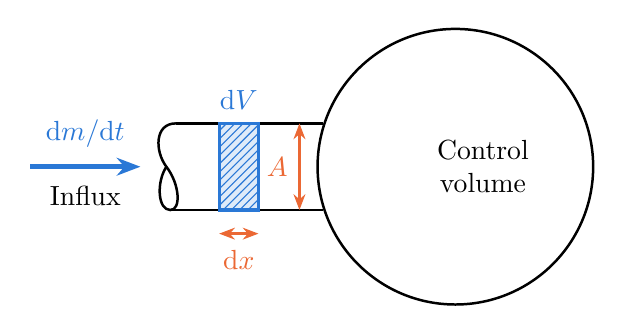
\begin{tikzpicture}[
    dim/.style={{Stealth[length=2mm]}-{Stealth[length=2mm]}, duRed, line width=0.9pt}]
  \def\r{0.55}
  % control volume
  \draw[line width=0.9pt] (5.0,0) circle (1.75);
  \node[align=center] at (5.35,0) {Control\\volume};
  % pipe (broken end on the left) running into the control volume
  \draw[line width=0.9pt] (1.45,\r) -- (3.32,\r);
  \draw[line width=0.9pt] (1.38,-\r) -- (3.32,-\r);
  \draw[line width=0.9pt] (1.45,\r) .. controls (1.18,\r) and (1.18,0.2) .. (1.33,0)
                                    .. controls (1.5,-0.22) and (1.52,-\r) .. (1.38,-\r)
                                    .. controls (1.22,-\r) and (1.2,-0.2) .. (1.33,0);
  % the fluid slice
  \fill[duBlue!15] (2.0,-\r) rectangle (2.5,\r);
  \fill[pattern=north east lines, pattern color=duBlue] (2.0,-\r) rectangle (2.5,\r);
  \draw[duBlue, line width=1.1pt] (2.0,-\r) rectangle (2.5,\r);
  \node[duBlue, anchor=south] at (2.25,\r+0.05) {$\mathrm{d}V$};
  % dimensions
  \draw[dim] (2.0,-\r-0.3) -- (2.5,-\r-0.3);
  \node[duRed, anchor=north] at (2.25,-\r-0.38) {$\mathrm{d}x$};
  \draw[dim] (3.02,-\r) -- (3.02,\r);
  \node[duRed, anchor=east] at (3.0,0) {$A$};
  % influx
  \draw[-{Stealth[length=3mm]}, duBlue, line width=1.8pt] (-0.4,0) -- (1.0,0);
  \node[duBlue, anchor=south] at (0.3,0.12) {$\mathrm{d}m/\mathrm{d}t$};
  \node[anchor=north] at (0.3,-0.12) {Influx};
\end{tikzpicture}
\end{document}
